\section{Geodetic Coordinates}\label{sec:coord}

\begin{figure}[H]
   \centering
    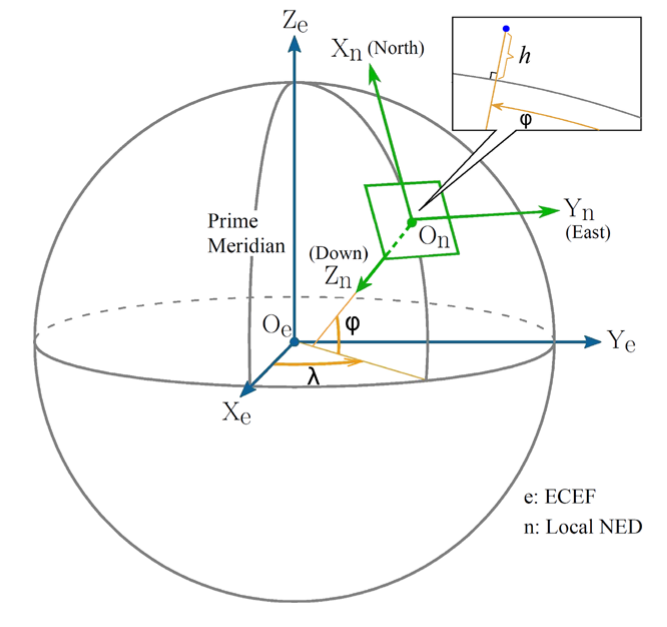
\includegraphics[width=.60\textwidth]{figures/GeoTemp1.png} 
    \label{fig:Geodetic}
    \caption{Geodetic, ECEF and local NED Frames.}  
\end{figure}

\paragraph{}The geodetic coordinate system is widely used in GPS-based navigation. Note that it is not an usual Cartesian coordinate system but a system that
characterizes a coordinate point near the earth’s surface in terms of longitude, latitude, and altitude (or height), which are respectively denoted by $\lambda$, $\varphi$, and h (yellow lines) in figure \ref{fig:Geodetic}.

\paragraph{}The \textit{World Geodetic System} is a standard used in cartography, geodesy and navigation. This standard sets reference points based on an ellipsoidal model of the earth and a gravitational equipotential surface that defines the nominal sea level. Its latest version is \textbf{WGS84}, and that is the one used throughout this project. 

The longitude measures the rotational angle (ranging from $-180$ to $180$ degrees) between the Prime Meridian and the measured point. The latitude measures the angle (ranging from $-90$ to $90$ degrees) between the equatorial plane and the normal of the reference ellipsoid that passes through the measured point. The height (or altitude) is the local vertical distance between the measured point and the reference ellipsoid.

\subsection{The Real Scenario}

IN PROGRESS...UNDER CONSTRUCTION

In mathematics, a spherical coordinate system is a coordinate system for three-dimensional space where the position of a point is specified by three numbers: the \textbf{radial distance} of that point from a fixed origin ($\rho$), its \textbf{polar angle} measured from a fixed zenith direction ($\theta$), and the \textbf{elevation angle} of its orthogonal projection on a reference plane, measured from a fixed reference direction on that plane ($\phi$).

\begin{figure}[H]
   \centering
    \includestandalone[width=.50\textwidth]{figures/3D_Sphcoord} 
    \label{fig:Spherical1}
    \caption{Spherical Coordinates}
\end{figure}

 It is necessary to define a unique set of spherical coordinates for each point, and therefore restricting their range is required. In our case the coordinates will be limited as follows:
\begin{align*}
& \rho \geq 0 \\
& -\pi \leq \theta < \pi \\
& \frac{-\pi}{2} \leq \phi \leq \frac{\pi}{2}
\label{eq:los_distToHorizon}
\end{align*} 

These constraints define the conversion between Cartesian and Spherical coordinates such that:
\begin{align*}
x &=  \rho\cos\phi\cos\theta  & \rho &= \sqrt{x^{2} + y^{2} + z^{2}} \\
y &= \rho\cos\phi\sin\theta   & \theta &= \text{atan2}\left(\frac{y}{x}\right)\\
z &= \rho\sin\phi       & \phi &=  \text{atan2}\left(\frac{z}{\sqrt{x^2 + y^2}}\right)
\label{eq:los_distToHorizon}
\end{align*} 

THIS SHOULD BE SOMEWHERE ELSE...MAYBE ANGLE SYSTEM ?????
\paragraph{} Once the coordinate system has been defined the general scenario of the project will be introduced.
\begin{figure}[H]
   \centering
    \includestandalone[width=.60\textwidth]{figures/Scenario1} 
    \label{fig:Scenario1}
    \caption{Representation of the general scenario.}
\end{figure}
where ($x_d,y_d,z_d$) are the coordinates that describe the position of the drone and ($x_{gs},y_{gs},z_{gs}$) are the coordinates that describe the position of the ground station.
The blue and green arrow represent the \textbf{antenna pointing vectors} of the ground station and drone, respectively.

\paragraph{} The \textbf{Line Of Sight (LOS) distance} is then given by the former defined variable $\rho$ and the \textbf{LOS angles} are given by the former defined variables $\theta$ and $\phi$.
\paragraph{} These angles will be referred during the rest of the text as \textit{optimal angles} or \textit{reference angles}, being $\theta_{GSopt}$ and $\phi_{GSopt}$ the corresponding to the Ground Station and $\theta_{Dopt}$ and $\phi_{Dopt}$ the analogous to the drone.
Note that the drone and the ground station antenna pointing vector, generally, will not be equal to the optimal angles. It is precisely our main task in this project to design a controller that drives these antennas to point to each other and, that way, we can get the best performance in the radio-communication link.


\begin{figure}[H]
   \centering
    \includestandalone[width=.60\textwidth]{figures/OptimalAngles1} 
    \label{fig:OptimalAngles1}
\end{figure}

\begin{figure}[H]
   \centering
    \includestandalone[width=.60\textwidth]{figures/OptimalAngles2} 
    \label{fig:OptimalAngles2}  
\end{figure}


As the next step, it is required to calculate the \textit{error angles}. This is the difference in both the $\theta$ and $\phi$ direction with respect to the optimal or LOS angles.
Note that, even though there is a clear relationship between the optimal angles for the ground station and the drone, the value is not exactly the same.

When aproaching this step, transforming the angles $\theta$ to the range $[0:2\pi]$ and $\phi$ to the range $[0:\pi]$ has proven to ease the calculations, ending up with the optimal angles described as:

\begin{equation}
  \theta_{GSopt}=
  \begin{dcases}
    {\rm atan2}\left(y_{d}-y_{gs}, x_{d}-x_{gs}\right), & \text{if } y_{d}\geq y_{gs}\\
    \pi + {\rm atan2}\left(y_{gs}-y_{d}, x_{gs}-x_{d}\right), & \text{if } y_{d} < y_{gs}
  \end{dcases}
\end{equation}

\begin{equation*}
  \phi_{GSopt}= 
  \dfrac{\pi}{2} - {\rm atan2}\left(z_{d}-z_{gs}, \sqrt{|x_{gs}-x_{d}|^{2}+|y_{gs}-y_{d}|^{2}}\right)
  \label{eq:OptGS}
\end{equation*}

\begin{equation}
  \theta_{Dopt}=
  \begin{dcases}
    \pi + {\rm atan2}\left(y_{d}-y_{gs}, x_{d}-x_{gs}\right), & \text{if } y_{d} \geq y_{gs}\\
    {\rm atan2}\left(y_{gs}-y_{d}, x_{gs}-x_{d}\right), & \text{if } y_{d} < y_{gs}
  \end{dcases}
\end{equation}

\begin{equation*}
  \phi_{Dopt}= 
  \dfrac{\pi}{2} + {\rm atan2}\left(z_{d}-z_{gs}, \sqrt{|x_{gs}-x_{d}|^{2}+|y_{gs}-y_{d}|^{2}}\right)
  \label{eq:OptD}
\end{equation*}

\paragraph{} Figures "Add 6 figures here" show the mentioned angles in order to fit the equations \ref{eq:OptGs} and \ref{eq:OptD}.

\paragraph{} !!!FIGURES!!
\begin{figure}[H]
   \centering
    \includestandalone[width=.60\textwidth]{figures/AnglesEx1} 
    \label{fig:OptimalAngles1}  
\end{figure}

\paragraph{} Finally, the LOS distance will be calculated as expected:
\begin{equation*}
  LOS_{distance}= 
  \sqrt{|x_{gs}-x_{d}|^{2}+|y_{gs}-y_{d}|^{2}+|z_{gs}-z_{d}|^{2}}
  \label{eq:OptD}
\end{equation*}

